%!TEX root = ../dissertation.tex
\begin{savequote}[75mm]
This is some random quote to start off the chapter.
\qauthor{Firstname lastname}
\end{savequote}

\chapter{Analisi e progettazione}

\section{Metodo di lavoro}
Dopo un'attenta analisi delle esigenze di questo progetto, la metodologia che abbiamo deciso di utilizzare è Agile Kanban. Questa metodologia, ci ha permesso di avere un'alta flessibilità sui task da svolgere, una visione ampia del progetto e il focus su una singola attività alla volta.
La metodologia Kanban è stata scelta anche per affrontare l'esiguo numero del team, composto da sole 2 persone, con effettivamente solo una che lavorava a pieno regime su di esso.
Questo perché rendeva un'ottima visione dell'insieme delle attività da svolgere, in progresso e già svolte, oltre a non necessitare di ruoli predefiniti come nell'\gls{Agile Scrum}
\paragraph{Metodologia kanban}
Fa parte della famiglia delle metodologie agile, alla base vi è l'utilizzo di una lavagna nella quale vi è specificato uno stato per ogni colonna presente.
\begin{figure}[h!]
	\centering
	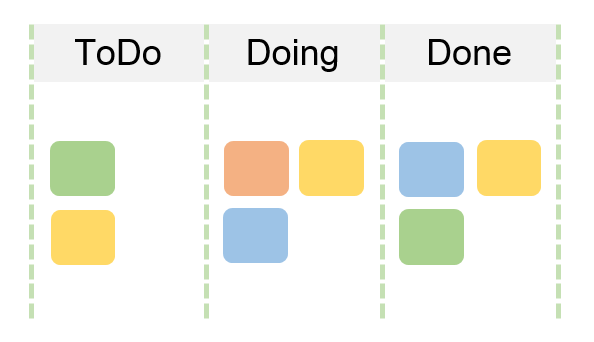
\includegraphics[scale=0.3]{figures/kanban-board}
	\caption[Short figure name.]{Esempio lavagna Kanban.
		\label{fig:logoGCP}}
\end{figure}	
Quello sopra riportato è uno degli esempi più semplici di lavagna Kanban, nella quale ogni task deve assumere tre stati per considerarsi completato "ToDo", "Doing" e "Done". Solitamente ogni componente del team ha la responsabilità di portare a completamente un solo task alla volta, così da evitare sovrapposizioni e confusione.
\\ 
Questa metodologia ha sicuramente giovato al progetto dato l'alto livello di flessibilità garantito e necessario al rispetto dalle richieste periodiche del cliente.
\section{Problemi affrontati}
Affrontare sfide, problemi e quesiti di carattere tecnologico, architetturale e implementativo è stata sicuramente la parte più formativa del periodo di stage, dato che in quelle situazioni lo studio autonomo e il confronto con esperti del settore come il mio Tutor sono stati di primaria importanza.
\\
I problemi affrontati durante questo progetto sono molteplici e vanno dall'analisi e scelta delle tecnologie da utilizzare all'integrazione tra le stesse.
\\
Per circoscrivere le problematiche abbiamo deciso di sviluppare il progetto in due sotto-progetti autonomi. 
Il primo tratta dell'ingestion dei dati e il secondo dell'utilizzo dei dati con il fine di categorizzare gli utenti. Da questi quindi, derivano diverse tipologie di problemi, tra cui la scelta e lo studio degli strumenti e delle \gls{best practices}.
\\
Il punto cruciale del sotto-progetto riguardante l'ingestion è stato lo studio delle tecnologie riguardanti Google Cloud Platform e con esso le conseguenti scelte obbligate, come lo studio di Apache Beam, l'utilizzo di sole librerie compatibili con Google Cloud ed i suoi strumenti.
\\
Per quanto riguarda la classificazione degli utenti, si è scelto di intraprendere una strada che potesse portare a dei vantaggi di utilizzo e portabilità, cioè si è deciso di utilizzare un \gls{container} Docker per lo sviluppo ed utilizzo degli algoritmi di classificazione.
Questo è stato fatto per agevolare l'installazione e configurazione in locale dell'intero pacchetto di strumenti da utilizzare, tra cui Spark, Kafka e Hadoop.
Ovviamente, l'utilizzo di Docker ha comportato la scelta del miglior compromesso per la creazione di un container adatto. Dato l'ampio pacchetto di strumenti da studiare in autonomia, abbiamo deciso quindi di utilizzare un \href{https://www.cloudera.com/documentation/enterprise/5-6-x/topics/quickstart_docker_container.html}{container Cloudera} già contenete la maggior parte degli strumenti necessari per sviluppare un processo di classificazione degli utenti.
Inoltre, per far si che i dati venissero continuamente aggiornati, come effettivamente succede nella fase di ingestion, abbiamo deciso di utilizzare Kafka Straming per mantenere un flusso continuo di verifica delle anomalie, così da mantenere in costante aggiornamento il cliente.

\section{Pianificazione del lavoro}
Durante i colloqui svolti con il tutor aziendale, è stato redatto il piano di lavoro. Ciò ha portato la suddivisione dello stage in 8 parti, ognuna della durata di una settimana.
    \begin{itemize}
	\item[] \textbf{Prima Settimana (40 ore)}
	\begin{itemize}
		\item Incontro con persone coinvolte nel progetto per discutere i requisiti e le richieste
		relativamente al sistema da sviluppare;
		\item Verifica credenziali e strumenti di lavoro assegnati;
		\item Presa visione dell’infrastruttura esistente;
		\item Formazione sulle tecnologie adottate;
	\end{itemize}
	\item[] \textbf{Seconda Settimana (40 ore)} 
	\begin{itemize}
		\item Comprensione strumenti di storicizzazione;
		\item Analisi funzionamento filesystem distribuito;
		\item Produzione script Python per produzione dati simulati;
	\end{itemize}
	\item[] \textbf{Terza Settimana (40 ore)} 
	\begin{itemize}
		\item Caricamento dati su filesystem distribuito;
		\item Securizzazione accesso ai dati;
		\item Studio teorico approccio statistico al problema;
	\end{itemize}
	\item[] \textbf{Quarta Settimana (40 ore)} 
	\begin{itemize}
		\item Comprensione strumenti di processamento;
		\item Analisi funzionamento RDD;
		\item Implementazione processo batch con Python e Spark;        
	\end{itemize}
	\item[] \textbf{Quinta Settimana (40 ore)} 
	\begin{itemize}
		\item Analisi funzionamento Dataframe;
		\item Implementazione processo di elaborazione Spark;
		\item Ingegnerizzazione soluzione batch;
	\end{itemize}
	\item[] \textbf{Sesta Settimana (40 ore)} 
	\begin{itemize}
		\item Test prestazionale processo spark;
		\item Tuning prestazionale;
		\item Studio applicazione real-time;
	\end{itemize}
	\item[] \textbf{Settima Settimana (40 ore)} 
	\begin{itemize}
		\item Storicizzazione dati su storage persistente;
		\item Studio funzionamento Kafka;
		\item Implementazione processo real-time con Spark Streaming;
	\end{itemize}
	\item[] \textbf{Ottava Settimana - Conclusione (40 ore)} 
	\begin{itemize}
		\item Costruzione layer accesso al dato persistente;
		\item Ingegnerizzazione soluzione Spark Streaming;
		\item Integrazione storage persistente;
	\end{itemize}
\end{itemize}
possibili diagrammi
\section{Risultati}
Alla fine del periodo di stage, i risultati ottenuti sono stati considerati più che positivi dal tutor aziendale Michele Giusto, dato che sono stati soddisfatti tutti i requisiti obbligatori e desiderabili. I requisiti facoltativi, non sono stati implementati per lasciare maggiore spazio e importanza ai requisiti obbligatori.
\\
Inoltre, il sotto-progetto riguardante la fase di ingestion ha avuto ottimi risultati, tale per cui si è dimostrata pronta per essere utilizzata in fasi di "produzione".
Per quanto riguarda la parte di classificazione, è stata messa a punto per scheletro e funzionalità senza però essere pronta per gestire effettivamente l'aggiornamento real time dei dati, soprattutto perché da parte del clienti vi è stato un rallentamento nel passaggio di dati ed informazioni per la scelta del miglior modello. 


